\documentclass[10pt]{beamer}
\usetheme{Rochester}
\usepackage[utf8]{inputenc}
\usepackage{amsmath}
\usepackage{amsfonts}
\usepackage{amssymb}
\usepackage[export]{adjustbox}
\setbeamertemplate{footline}[frame number]
\author{Justin Anguiano}
\title{Performance Optimization}
%\setbeamercovered{transparent} 
%\setbeamertemplate{navigation symbols}{} 
%\logo{} 
%\institute{} 
%\date{} 
%\subject{} 
\begin{document}

\begin{frame}
\titlepage
\end{frame}

%\begin{frame}
%\tableofcontents
%\end{frame}

\begin{frame}{}
Goal --- Improve Physics analysis performance \\
\quad \quad \\
Use different C/Python approaches to obtain a low programming overhead but high performance\\ 
\end{frame}

\begin{frame}
\textbf{Task to be optimized: Read File(s) containing a TTree, produce histograms from elements of the tree(s), write histograms to a TFile}\\
\quad \quad \\
\scriptsize
\textbf{ Three histograms are produced: TH1D: track $p_{T}$ weighted by $1/p_{T}$, TH1D: track $p_z$, TH2D, track $p_x$ vs $p_y$} \\
\normalsize
\quad \quad \\
First attempt using ROOT6 parallelization on local machine (laptop)\\
methods:\\
\begin{itemize}
\item Sequential run over a test file with TTreeReader (Compiled and Interpreted)
\item Parallelized run over a test file with TTreeReader (Compiled and Interpreted)
\end{itemize}

Test File Details\\
\begin{itemize}
\item code adapted from example: \url{https://root.cern.ch/doc/v612/imt101__parTreeProcessing_8C.html} 
\item uses fake event file containing 48000 events; each with some number of tracks per event
\item total tracks overall $\approx 2.4e+7$ 
\end{itemize}

\end{frame}


\begin{frame}
First Test Results:\\
\begin{columns}
	\begin{column}{0.5\textwidth}
	\begin{itemize}
		\scriptsize
		\item Time is Mean time $\pm$ stdev over 10 trials
		\item no guarantee of system releasing requested resources (nthreads) so perform multiple trials
		\item data point at nThreads = 0 is the basic sequential program
		\item high threadcount performance possibly bottlenecked by system?
		\item Takeaway: Compiling is important! $\approx $Factor of 2 improvement
	\end{itemize}
	\end{column}
	\begin{column}{0.5\textwidth}
   		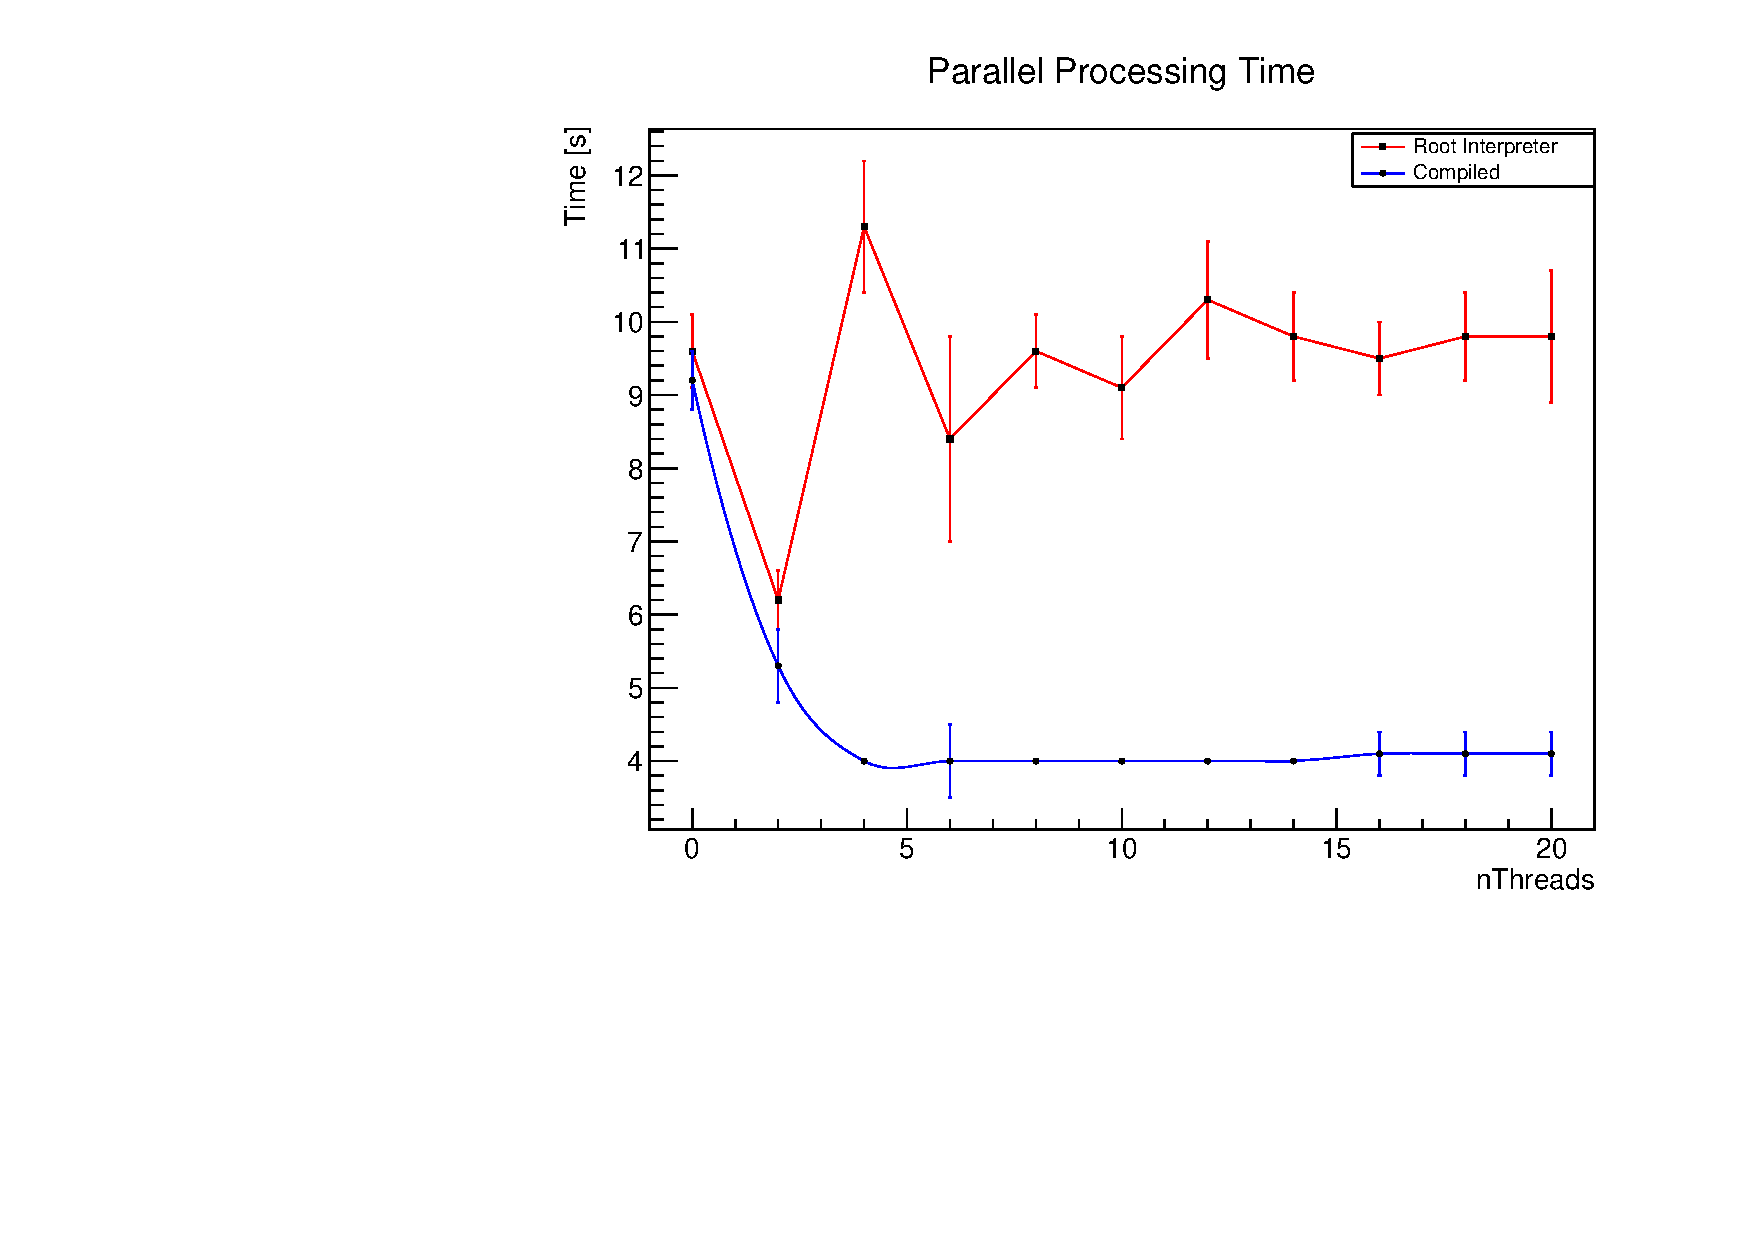
\includegraphics[scale=0.3, left]{../ParTree/test1plot.pdf}

	\end{column}
\end{columns}
\end{frame}

\begin{frame}
Second attempt using ROOT6 parallelization, classic(Make Class) parallelization, MultiProcessing on t3.unl.edu\\
methods:\\
\begin{itemize}
\item Sequential run over multiple test files with TTreeReader (Compiled and Interpreted)
\item Parallelized run over multiple test files with TTreeReader (Compiled and Interpreted)
\item Sequential run over multiple test files with Make Class (Compiled and Interpreted)
\item Parallelized run over multiple test files with Make Class (Compile and Interpreted)
\end{itemize} 

Test File set Details:\\
\begin{itemize}
\item using 10 files from Single Muon 2018 dataset
\item X events each with at least 1 conversion per event
\item total tracks overall = Y
\end{itemize}

\end{frame}



\end{document}